\documentclass[conference]{IEEEtran}
\usepackage[T1]{fontenc}
\renewcommand{\ttdefault}{lmtt}
\usepackage{amsmath,amssymb,booktabs,graphicx,microtype,xcolor,url}
\usepackage{tikz}
\usetikzlibrary{arrows.meta,positioning}
\usepackage[hidelinks]{hyperref}
\hypersetup{pdftitle={Bad Blood V2 - Final Results 20261013},pdfauthor={Jingyi Guo}}
\pagestyle{plain}
\setlength{\emergencystretch}{1.5em}
\newcommand{\pair}{\textsc{PairSE}}
\newcommand{\pkg}{\texttt{final\_results\_20261013}}
\title{Bad Blood V2: Attention-Based Population Models\protect\\and Reference-Conditioned Personalization}
\author{\IEEEauthorblockN{Jingyi Guo}
\IEEEauthorblockA{Bad Blood Project, University of Notre Dame\\
Research and Engineering Results Report --- October 13, 2026}}
\begin{document}
\maketitle
\thispagestyle{plain}
\begin{abstract}
This report consolidates the trained models and completed evaluations of Bad
Blood V2. A compact residual one-dimensional convolutional network with
final-stage squeeze-and-excitation (CNN+SE) estimates systolic and diastolic
blood pressure (SBP/DBP) from ten-second physiological signal windows. Matched
ECG+PPG and PPG-only versions are retained. Source training uses 390,600
segments from 1,085 participants in the VitalDB-derived partition of PulseDB.
Three-seed main-test participant-macro MAE is 12.39/8.00 mmHg for ECG+PPG and
12.32/7.85 for PPG-only. Reference-conditioned personal adaptation learns a
pressure change relative to known early personal measurements. With matched
calibration data, both versions improve upon personal mean in both pressures
for every seed in the six-person and sixteen-person target cohorts. Dual-input
personalization also improves upon bias correction for both pressures in every
seed in the six-person cohort, reaching 8.32/3.76 mmHg. That joint advantage
does not fully transfer to the sixteen-person cohort, where bias correction
remains stronger for DBP. We provide architecture definitions, fitting details,
complete error metrics, controls, checkpoint files and runnable inference.
\end{abstract}
\begin{IEEEkeywords}
blood pressure, PPG, ECG, squeeze-and-excitation, calibration, personalization
\end{IEEEkeywords}

\section{Release decisions and contribution}
The engineering objective is to obtain compact population and personalized
estimators that can use newly observed physiological signals. This report
records the \emph{20261013 final V2 snapshot}, not a new training run or a claim
that every scientific hypothesis succeeded. It contains two reusable outcomes.

\textbf{Population model.} We retain high-resolution residual CNN+SE with
38,296 parameters in two input configurations. ECG+PPG is the primary
configuration within this family because its three-seed validation score and
pressure-range stress-test result are better. PPG-only is a useful single-sensor
alternative with slightly lower main-test MAE. The three-seed architecture-wide
validation comparison originally selected the plain CNN, whereas SE had the
lowest observed test MAE among its six required architecture candidates. The
retained SE research model should not be described as winning both rankings.

\textbf{Personal model.} We retain \pair, a reference-conditioned pressure-change
model built on the same CNN+SE. Both modalities beat personal mean across all
three seeds and both target cohorts. Dual-input \pair\ provides the clearest
six-person evidence of simultaneous improvement over mean and bias correction;
PPG-only has lower personal-development error and slightly lower average
sixteen-person \pair\ error. There is no demonstrated universal input-mode
winner. Both learned models and both simple controls remain in the package.

\section{Data, task and information boundaries}
PulseDB combines cleaned ECG, PPG and invasive arterial pressure signals from
VitalDB and MIMIC-III \cite{wang2023pulsedb}. Our experiments use its
\emph{VitalDB-derived population partition and individual-record files}, not
the whole combined collection. Each model input is a synchronized ten-second
window sampled at 125 Hz; each output is one SBP and one DBP in mmHg. The label
comes from the arterial-pressure reference. ABP samples, current BP labels,
demographics and participant IDs are not population prediction inputs.

\begin{table}[t]\centering
\caption{Fixed population partitions after participant exclusions.}
\label{tab:data}\small
\begin{tabular}{lrr}\toprule
Partition & Participants & Segments\\\midrule
Training & 1,085 & 390,600\\
Validation & 192 & 69,120\\
Main test & 141 & 56,400\\
AAMI-designated stress subset & 116 & 666\\\bottomrule
\end{tabular}\end{table}

The corrected population split excludes historically explored personal subjects;
the subsequent personal cohort is also checked for disjointness. The AAMI
subset is evaluated separately and is not added to the main-test count as an
independent experiment. Its name refers to the dataset construction, not
certification of our estimator. Previously evaluated test cohorts are retained
for controlled comparison; they are not presented as untouched external tests.

Personalization uses four development participants to choose settings and two
target cohorts: the original six and a subsequent sixteen. The original six
provide 4,284 later query windows; the sixteen provide 2,310. The sixteen were
unseen at their first evaluation but had already been examined before this
modality study. Cohorts are therefore reported separately, not combined into
an apparently new validation population. The support is all eligible windows
in the first 20\% of elapsed recording time, with a ten-second guard before
later query windows. Gaps in the recording clock are retained. These dense
public-data references are not actual cuff events or ND measurements.

\section{Population architecture and training}
\subsection{Signal representation and network}
The supplied filtered ECG and PPG fields are scaled independently within each
window to the unit interval. The tensor shape is $N\times2\times1250$, ordered
ECG then PPG. The PPG-only fit is trained from scratch without ECG. An internal
mask zeros ECG in both ordinary forward inference and reference encoding.
Keeping the two-slot representation maintains a controlled parameter-matched
comparison; it is not a claim that ECG is needed for the PPG model.

\begin{table}[t]\centering\small
\caption{CNN+SE architecture; shapes omit batch dimension.}
\label{tab:layers}
\begin{tabular}{lp{2.45in}}\toprule
Stage & Operation and output\\\midrule
Input & 2 channels $\times$ 1,250 samples; no initial decimation\\
Stem & Conv1d 2$\to$8, kernel 7, stride 2, pad 3; BN; SiLU. $8\times625$\\
Block1 & Residual 8$\to$16, stride 2. $16\times313$\\
Block2 & Residual 16$\to$32, stride 2. $32\times157$\\
Block3 & Residual 32$\to$48, stride 2. $48\times79$\\
SE gate & Temporal mean; Linear 48$\to$6; ReLU; Linear 6$\to$48; sigmoid; multiply channels\\
Readout & Global temporal mean; dropout 0.15; Linear 48$\to$32; SiLU; Linear 32$\to$2\\\bottomrule
\end{tabular}\end{table}

Each residual block has a kernel 7 convolution, BN and SiLU, followed by a
kernel 5 convolution and BN. A stride-matched kernel 1 projection and BN form
the skip branch; SiLU follows the sum. The SE mechanism \cite{hu2018se}
reweights learned feature channels after the final residual stage. These
channels mix signal features; their weights are not direct sensor importance
scores. CBAM and temporal-only attention were also compared using the same
backbone. Adding SE increases parameters from 37,666 to 38,296, about 1.7\%.

\subsection{Objective, optimizer and checkpoint selection}
For normalization $N(\cdot)$, the physical-unit population prediction is
\begin{equation}
 p(X)=\mu+\sigma\odot f_\theta(N(X)),
\end{equation}
where training-only label center $\mu=(115.41765,62.92810)$ and scale
$\sigma=(18.94188,12.08322)$ are stored in the checkpoint. The objective is
mean squared error in standardized SBP/DBP, not a mixture of test metrics.
Both modes use AdamW, learning rate 0.001, weight decay 0.001, batch 256, input
noise SD 0.003 and gradient-norm clipping at 5. A plateau scheduler halves the
learning rate after three validation non-improvements. Maximum training is 40
epochs, with early-stopping patience 8. Checkpoints minimize the mean of SBP
and DBP participant-macro validation MAE. All six SE fits stopped after nine
epochs and retained epoch 1 (Table~\ref{tab:epochs}); later epochs were evaluated
but did not improve that criterion. Seeds 42,43,44 quantify training variation.
Seed 42 is the representative within each modality because its validation score
is best, not because of a test-set ranking.

\begin{table}[t]
\centering\caption{Population fits: completed epochs and validation-selected checkpoint.}\label{tab:epochs}
\scriptsize
\setlength{\tabcolsep}{4pt}
\begin{tabular}{lrrrr}\toprule
Input & Seed & Run epochs & Best epoch & Val. score\\\midrule
dual & 42 & 9 & 1 & 10.291\\
dual & 43 & 9 & 1 & 10.457\\
dual & 44 & 9 & 1 & 10.421\\
ppg & 42 & 9 & 1 & 10.374\\
ppg & 43 & 9 & 1 & 10.583\\
ppg & 44 & 9 & 1 & 10.406\\
\bottomrule\end{tabular}
\end{table}

\begin{table}[t]
\centering\caption{Dual-input architectures: three-seed participant-macro MAE (SBP / DBP), mmHg. Bold: lowest per pressure and split.}\label{tab:architecture}
\scriptsize
\setlength{\tabcolsep}{4pt}
\begin{tabular}{lrrr}\toprule
Model & Parameters & Validation & Main test\\\midrule
Plain CNN & 37666 & \textbf{12.41} / 8.33 & 12.59 / 8.36\\
CNN+SE & 38296 & 12.51 / \textbf{8.26} & \textbf{12.39} / \textbf{8.00}\\
CNN+temporal & 37680 & 12.49 / 8.32 & 12.58 / 8.31\\
CNN+CBAM & 38310 & 12.52 / 8.29 & 12.42 / 8.11\\
CNN+additive & 38296 & 12.44 / 8.34 & 12.66 / 8.18\\
CNN+SE-all & 38670 & 12.47 / 8.32 & 12.49 / 8.23\\
\bottomrule\end{tabular}
\end{table}


\section{Reference-conditioned personalization}
\subsection{Model definition}
Directly fitting all population parameters on a small personal reference bank
did not reliably improve the simple controls. \pair\ instead makes known
reference BP an explicit input and learns waveform-dependent pressure changes.
This follows the general reference-conditioning and layer-selective transfer
ideas in prior work \cite{schlesinger2020,leitner2022}, implemented here with
our matched CNN+SE and chronological evaluation.

The shared encoder produces $h_c,h_r\in\mathbb R^{48}$ and standardized
population predictions $p_c,p_r\in\mathbb R^2$ for current and reference
windows. Features are standardized using source-training feature statistics.
With known standardized reference pressure $y_r$, define
\begin{align}
 z_{cr}&=[h_c-h_r,\ h_r,\ y_r,\ p_c-p_r],\\
 z_{rr}&=[0,\ h_r,\ y_r,\ 0],\\
 \widehat y_{c\mid r}&=y_r+(p_c-p_r)+g_\phi(z_{cr})-g_\phi(z_{rr}).
\end{align}
The change network $g_\phi$ is a 100$\to$64$\to$32$\to$2 MLP with SiLU between
layers and 8,610 parameters. Its last layer starts at zero during source
training. The full shared-encoder model has 46,906 parameters; personal fitting
updates only the 8,610 change-head parameters. The subtraction anchors identical
current/reference waveforms to their known reference pressure. Final inference
averages $\widehat y_{c\mid r}$ over \emph{all} early references and converts
back to mmHg. Current or later reference BP is never passed to inference.

\begin{figure*}[t]\centering
\resizebox{\textwidth}{!}{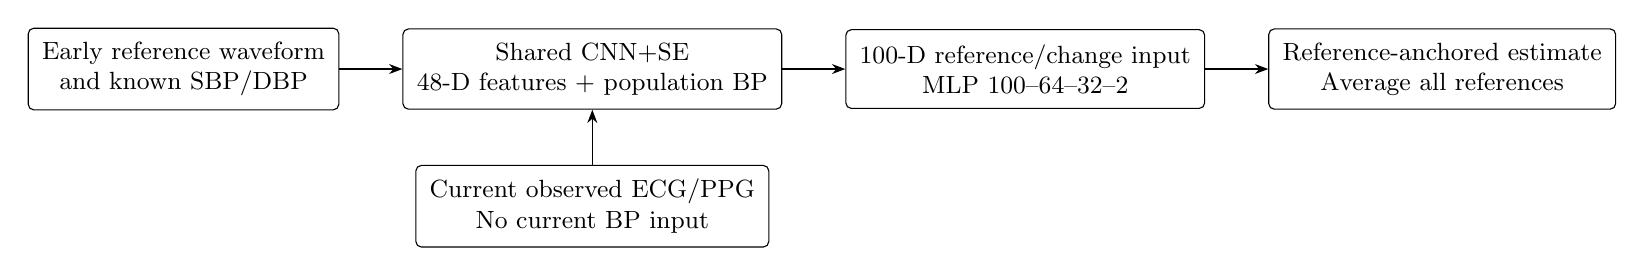
\begin{tikzpicture}[font=\small,node distance=7mm and 8mm,
 box/.style={draw,rounded corners=2pt,align=center,minimum height=10mm,inner sep=5pt},
 >=Stealth]
\node[box] (ref) {Early reference waveform\\and known SBP/DBP};
\node[box,right=of ref] (enc) {Shared CNN+SE\\48-D features + population BP};
\node[box,right=of enc] (delta) {100-D reference/change input\\MLP 100--64--32--2};
\node[box,right=of delta] (out) {Reference-anchored estimate\\Average all references};
\node[box,below=of enc] (cur) {Current observed ECG/PPG\\No current BP input};
\draw[->] (ref)--(enc);\draw[->](enc)--(delta);\draw[->](delta)--(out);
\draw[->](cur)--(enc);
\end{tikzpicture}}
\caption{\pair\ inference. The reference bank belongs to the same person and
precedes the evaluated query period. Source-trained representation and
personalized change head are shared across all reference/query pairs.}
\label{fig:pair}
\end{figure*}

\subsection{Source pair training and personal fitting}
Source pair-head training freezes the CNN+SE and uses all 390,600 source
training windows. A random non-self window from the same source participant
serves as each reference; source subset timestamps are not recoverable, so
this stage is not a source chronological forecasting experiment. The head uses
Adam lr 0.001, batch 2,048, standardized MSE, clipping 5, up to 20 epochs and
validation patience 5. Source feature centering/scaling is fixed thereafter.

Personal development compares no adaptation and eight combinations of scope
(head-only/full), learning rate(0.0003/0.001) and steps(25/100). It minimizes
the worst of the four development MAE ratios to personal mean and bias
correction, with mean MAE as tie-breaker. Settings are chosen independently
for each modality, averaging seeds on the same four development people;
both choose \textbf{head-only Adam, lr 0.0003,25 steps}. This selection does
not assume every development baseline is beaten: dual development SBP is
7.53 versus 6.76 for bias correction; PPG development is 7.23/4.30 versus
9.17/5.43 for bias correction and 12.53/5.26 for personal mean.

All eligible early support windows participate in at least one time-separated
pair. Each fitting step uses all valid chronological support pairs, and only
support labels enter the loss. BatchNorm running statistics and dropout stay
fixed; there is no personal weight decay or L2-SP penalty. The frozen encoder
choice is empirical, not an imposed requirement to keep personalization small.
Later query labels are used only for evaluation, not stopping or tuning.

\subsection{Fair controls}
Every method receives the same reference bank $S_i$ and query set $Q_i$ for
participant $i$. The personal mean needs no query waveform:
\begin{equation}
 \widehat y^{\rm mean}_{iq}=|S_i|^{-1}\sum_{r\in S_i}y_{ir}.
\end{equation}
The stronger additive control uses the same modality's pretrained predictor:
\begin{equation}
 \widehat y^{\rm bias}_{iq}=p(X_{iq})+
 |S_i|^{-1}\sum_{r\in S_i}\{y_{ir}-p(X_{ir})\}.
\end{equation}
Bias correction already tracks the population model's within-person changes;
it is not equivalent to predicting a constant. \pair\ must improve the learned
change relationship, not simply recover the person's typical BP.

\section{Metrics and comparisons}
Let $e_{ij}=\widehat y_{ij}-y_{ij}$. We report MAE, RMSE, signed mean error
(Bias), sample error SD with denominator $n-1$, and fractions with
$|e|\leq5,10,15$ mmHg. Participant-macro metrics compute each person's metric
and then weight people equally. Pooled metrics treat every window equally.
Macro SD averages within-person SD and excludes some between-person offsets;
it must not be substituted for pooled SD. Each pressure is evaluated separately.

All main tables average the metrics of three separately trained/evaluated
seeds, not an ensemble's predictions. Paired confidence intervals resample
people after averaging each person's matched-seed difference. Repeated seeds
are not independent participants. Per-person MAE, tail errors, pressure strata,
correlations and $R^2$ are also retained in the machine-readable results.

\subsection{Population results}
Table~\ref{tab:architecture} provides the architecture comparison. Plain CNN
test MAE is 12.59/8.36; SE is 12.39/8.00 and CBAM is 12.42/8.11. Plain CNN
has the best mean validation score 10.371, narrowly ahead of SE10.390;
therefore the test improvement is an observed comparison, not validation proof
of SE dominance. The new matched modality study uses the same three seeds
and source data for both SE models. Dual validation MAE is 12.51/8.26;
PPG-only is 12.50/8.41. Main-test PPG-only MAE is 12.32/7.85, but its signed
bias is more negative. On the AAMI-designated subset, macro MAE is 19.99/12.62
for dual and 20.80/13.19 for PPG. This motivates retaining both input modes
and using dual as the population default rather than declaring PPG universally
better. Table~\ref{tab:population} provides all requested pooled metrics.

\subsection{Where personalization beats both controls}
On the original six people, dual \pair\ gives 8.32/3.76 versus 9.47/4.22 for
mean and 9.16/4.40 for bias correction. The relative improvements over bias
correction are 9.2\% for SBP and 14.6\% for DBP. Each of the three seeds
improves both endpoints against both controls. Seed-averaged per-person
improvement over bias correction occurs in five of six people for each
endpoint. Descriptive paired MAE-difference 95\% intervals are
$[-1.46,-0.23]$ for SBP and $[-0.95,-0.29]$ for DBP. The joint primary-MAE
criterion is therefore met on this cohort.

The PPG version also improves the six-person average to 8.19/3.85, but its
SBP advantage over PPG bias correction is only 0.08 mmHg and appears in one
of three seeds. Some threshold metrics do not improve even where MAE does;
the complete tables preserve these differences.

\subsection{Expanded-cohort result}
On sixteen people, dual \pair\ reaches 12.67/7.61 and PPG \pair\ reaches
12.47/7.51, both better than mean 17.41/9.71. This improvement holds for
SBP and DBP in every seed. However, the own-modality bias controls reach
12.82/7.48 (dual) and 12.74/6.89 (PPG). PPG \pair\ improves macro SBP
in all three seeds but worsens DBP in all three. Dual improves SBP in two
of three and DBP in one of three. Table~\ref{tab:seeds} shows every seed.

For PPG, paired mean-baseline differences are$-4.95/-2.20$ mmHg, with
95\% intervals$[-8.09,-1.52]$ and$[-3.53,-0.92]$. Against bias correction,
differences are$-0.27/+0.63$, with intervals$[-2.12,1.53]$ and$[-0.04,1.26]$.
PPG-versus-dual \pair\ intervals cross zero for both pressures. Neither
input modality establishes a stable overall winner in this cohort.

Pooled results also matter. PPG \pair\ reduces pooled Bias from 2.72/1.92
to$-0.25/0.37$ relative to bias correction, but pooled SD increases from
14.49/8.03 to 15.28/9.15 and MAE increases from 12.03/6.58 to 12.34/7.30.
The small macro SBP gain reverses when weighting windows rather than people.
Lower aggregate signed bias alone is not evidence of lower prediction error.

\subsection{Follow-up calibration and retained method}
The completed residual follow-up evaluated twenty centered linear/kernel
calibration configurations and support-only forward validation, using the
same references and three seeds. Settings were selected on the four
development people before target evaluation. The dual selection used a
feature RBF residual correction for SBP and prediction-feature linear ridge
for DBP; PPG selection retained the previous \pair\ for both outputs.
The new dual sixteen-person MAE is 12.34/8.23, versus 12.67/7.61 for \pair;
its six-person result is 9.87/4.43 versus 8.32/3.76. Better SBP does not
satisfy the joint criterion when DBP worsens. We therefore retain \pair\ and
archive the full negative follow-up rather than silently changing one
endpoint after inspecting target results.

\section{Implementation and reproducibility}
The \href{https://github.com/place-bot/Bad-Blood/tree/research/v2-vitaldb-attention-personalization/model\%20training/v2/final_results_20261013}{GitHub final-results folder} separates \texttt{01\_pretrained} and
\texttt{02\_personalization}. It contains six population checkpoints, six
source pair-head checkpoints and 132 participant-specific checkpoints
($22\times3\times2$). The shared implementation includes the exact backbone,
modality mask and pair architecture, a portable inference loader and the fixed
personal adaptation routine. Source snapshots and full-study instructions
preserve the original fitting procedures. Checkpoints include label
normalization statistics; PairSE also stores feature normalization.

For a new participant, start from that modality's source PairSE checkpoint,
fit only on early known references, and supply the same reference bank during
later prediction. A different person's fitted checkpoint is not a generic
deployable personal model. PPG inference may accept $N\times1\times1250$;
the wrapper inserts the zero ECG slot. Raw, unfiltered arbitrary sensor data
are not accepted as though already matched to the training representation.

The experiment verification covered 816 units and replayed 39,564 target
predictions exactly in the recorded environment. The residual follow-up
verified 1,260 units with maximum replay difference$1.53\times10^{-5}$ mmHg.
Release checks load every packaged checkpoint, compare the portable loader
with the original inference, and check the selected personal fit and
ECG-invariance of the PPG path. These checks concern software correctness,
not new generalization evidence. Git records, artifact SHA256 hashes, complete
per-person metrics and the editable report are included.

The population model is compact (about 150 KiB of float32 parameter values,
excluding buffers/container metadata). Local recorded dual seed 42 CPU
batch-one median inference was 1.48 ms over 20 repetitions. This is a development
computer timing, not a Raspberry Pi benchmark. PairSE can cache all reference
embeddings so reference signals need not be re-encoded on every update;
latency and memory on the final device still require measurement.

\section{Conclusion}
V2 delivers two compact population input modes and an explicit,
reference-conditioned personal model. The six-person dual-input result
demonstrates simultaneous improvement over personal mean and additive bias
correction across seeds. Expanded evaluation confirms improvement over personal
mean, while identifying bias correction as a strong DBP comparator. The final
package preserves both findings and supplies the models needed to reproduce
them. The next scientifically useful comparison is a larger personal
development cohort with a newly reserved target cohort, followed by separately
evaluated ND sensor/cuff transfer. The present results estimate scalar current
BP from observed signals; they are neither future-ABP-waveform forecasts nor
clinical-device validation.

\bibliographystyle{IEEEtran}
\bibliography{references}
\clearpage
\begin{table*}[t]
\centering\caption{Population pooled metrics, averaged across three seeds. All pressure pairs are SBP / DBP. Thresholds are absolute errors in mmHg; SD uses N-1. Bold: best per pressure within each split.}\label{tab:population}
\footnotesize
\setlength{\tabcolsep}{4pt}
\begin{tabular}{lrrrrrrr}\toprule
Split / input & MAE & RMSE & Bias & SD & Within 5 (\%) & Within 10 (\%) & Within 15 (\%)\\\midrule
validation / dual & 12.51 / \textbf{8.26} & 15.95 / \textbf{10.55} & \textbf{-1.19} / \textbf{-0.03} & 15.90 / \textbf{10.54} & \textbf{26.13} / \textbf{37.91} & \textbf{48.54} / \textbf{67.08} & 66.09 / \textbf{85.17}\\
validation / ppg & \textbf{12.50} / 8.41 & \textbf{15.92} / 10.71 & -1.43 / -0.72 & \textbf{15.83} / 10.62 & 25.39 / 37.28 & 48.35 / 66.37 & \textbf{66.64} / 84.30\\
test / dual & 12.39 / 8.00 & 15.89 / 10.19 & \textbf{-1.76} / \textbf{-0.89} & 15.78 / 10.15 & \textbf{26.03} / \textbf{38.83} & \textbf{49.22} / 68.91 & 67.60 / 86.68\\
test / ppg & \textbf{12.32} / \textbf{7.85} & \textbf{15.73} / \textbf{9.88} & -2.05 / -1.64 & \textbf{15.57} / \textbf{9.67} & 25.52 / 38.39 & 48.67 / \textbf{69.38} & \textbf{67.82} / \textbf{87.85}\\
aami / dual & \textbf{19.46} / \textbf{12.42} & \textbf{26.33} / \textbf{16.14} & \textbf{-13.22} / \textbf{-8.21} & \textbf{22.76} / 13.90 & 17.82 / \textbf{25.23} & \textbf{35.79} / \textbf{49.65} & \textbf{51.75} / \textbf{69.92}\\
aami / ppg & 20.10 / 12.99 & 27.16 / 16.47 & -13.95 / -9.11 & 23.30 / \textbf{13.69} & \textbf{19.22} / 22.87 & 35.59 / 45.80 & 50.35 / 67.17\\
\bottomrule\end{tabular}
\par\smallskip\begin{minipage}{\textwidth}\footnotesize Table notation: bold marks the best value per SBP/DBP in the stated comparison group: lower MAE, RMSE and SD, Bias closest to zero, and higher within-threshold percentages. Comparisons use unrounded values; numerical ties are all bold. Bold does not imply statistical significance or determine model selection.\end{minipage}
\end{table*}

\begin{table*}[t]
\centering\caption{Original six people: macro metrics, three-seed average. Pairs are SBP / DBP; errors in mmHg. Macro SD averages within-person sample SD.}\label{tab:historical_six_macro}
\footnotesize
\setlength{\tabcolsep}{4pt}
\begin{tabular}{lrrrrrrr}\toprule
Split / input & MAE & RMSE & Bias & SD & Within 5 (\%) & Within 10 (\%) & Within 15 (\%)\\\midrule
dual / Mean & 9.47 / 4.22 & 12.19 / 5.46 & 0.50 / -0.95 & 11.14 / 4.82 & 35.72 / 68.34 & 64.56 / 92.32 & 80.14 / 97.75\\
dual / Bias correction & 9.16 / 4.40 & 11.23 / 5.27 & 0.60 / -0.46 & 9.35 / 4.25 & 33.26 / 62.42 & 63.41 / 93.89 & 81.90 / 99.53\\
dual / PairSE & 8.32 / 3.76 & 10.27 / 4.69 & 0.98 / -0.53 & 9.07 / 4.11 & 36.65 / 71.51 & 68.06 / 95.53 & 86.12 / 99.28\\
ppg / Mean & 9.47 / 4.22 & 12.19 / 5.46 & 0.50 / -0.95 & 11.14 / 4.82 & 35.72 / 68.34 & 64.56 / 92.32 & 80.14 / 97.75\\
ppg / Bias correction & 8.27 / 4.28 & 10.31 / 5.34 & -1.49 / -1.83 & 8.49 / 4.15 & 39.01 / 63.42 & 68.40 / 93.20 & 85.32 / 99.11\\
ppg / PairSE & 8.19 / 3.85 & 10.17 / 4.83 & -1.89 / -1.79 & 8.66 / 4.26 & 37.68 / 70.85 & 68.21 / 94.91 & 86.24 / 99.11\\
\bottomrule\end{tabular}
\end{table*}

\begin{table*}[t]
\centering\caption{Subsequent sixteen people: macro metrics, three-seed average. Pairs are SBP / DBP; errors in mmHg. Macro SD averages within-person sample SD.}\label{tab:previous_sixteen_macro}
\footnotesize
\setlength{\tabcolsep}{4pt}
\begin{tabular}{lrrrrrrr}\toprule
Split / input & MAE & RMSE & Bias & SD & Within 5 (\%) & Within 10 (\%) & Within 15 (\%)\\\midrule
dual / Mean & 17.41 / 9.71 & 19.56 / 10.87 & 3.23 / 3.02 & 11.18 / 5.73 & 15.06 / 23.73 & 28.68 / 57.18 & 42.71 / 81.01\\
dual / Bias correction & 12.82 / 7.48 & 14.60 / 8.56 & 5.19 / 3.11 & 8.38 / 4.83 & 21.87 / 40.94 & 42.33 / 69.61 & 61.71 / 91.21\\
dual / PairSE & 12.67 / 7.61 & 14.58 / 8.72 & 2.93 / 1.78 & 9.18 / 4.92 & 27.74 / 40.67 & 48.45 / 72.59 & 62.60 / 89.10\\
ppg / Mean & 17.41 / 9.71 & 19.56 / 10.87 & 3.23 / 3.02 & 11.18 / 5.73 & 15.06 / 23.73 & 28.68 / 57.18 & 42.71 / 81.01\\
ppg / Bias correction & 12.74 / 6.89 & 14.33 / 7.95 & 4.55 / 2.73 & 8.07 / 4.57 & 20.55 / 42.05 & 40.49 / 76.80 & 63.05 / 93.28\\
ppg / PairSE & 12.47 / 7.51 & 14.07 / 8.60 & 2.63 / 1.61 & 8.78 / 4.81 & 26.39 / 38.33 & 46.45 / 70.90 & 63.59 / 88.89\\
\bottomrule\end{tabular}
\end{table*}

\clearpage
\begin{table*}[t]
\centering\caption{Every personal seed: participant-macro MAE (SBP / DBP), mmHg. The reference-only mean is deterministic, not three independent replications. Bold: best method per pressure within each row.}\label{tab:seeds}
\footnotesize
\setlength{\tabcolsep}{4pt}
\begin{tabular}{lrrrrr}\toprule
Cohort & Input & Seed & Personal mean & Bias correction & PairSE\\\midrule
Six & dual & 42 & 9.47 / 4.22 & 9.00 / 4.35 & \textbf{7.59} / \textbf{3.73}\\
Six & dual & 43 & 9.47 / 4.22 & 9.91 / 4.66 & \textbf{9.05} / \textbf{3.96}\\
Six & dual & 44 & 9.47 / 4.22 & 8.58 / 4.20 & \textbf{8.32} / \textbf{3.58}\\
Six & ppg & 42 & 9.47 / 4.22 & \textbf{7.85} / 4.37 & 8.07 / \textbf{3.95}\\
Six & ppg & 43 & 9.47 / 4.22 & \textbf{8.57} / 4.22 & 8.63 / \textbf{4.04}\\
Six & ppg & 44 & 9.47 / 4.22 & 8.40 / 4.24 & \textbf{7.88} / \textbf{3.55}\\
Sixteen & dual & 42 & 17.41 / 9.71 & \textbf{12.68} / \textbf{7.49} & 12.78 / 7.73\\
Sixteen & dual & 43 & 17.41 / 9.71 & 12.78 / 7.57 & \textbf{12.62} / \textbf{7.50}\\
Sixteen & dual & 44 & 17.41 / 9.71 & 13.00 / \textbf{7.36} & \textbf{12.62} / 7.60\\
Sixteen & ppg & 42 & 17.41 / 9.71 & 12.68 / \textbf{6.85} & \textbf{12.40} / 7.29\\
Sixteen & ppg & 43 & 17.41 / 9.71 & 12.91 / \textbf{6.94} & \textbf{12.42} / 7.68\\
Sixteen & ppg & 44 & 17.41 / 9.71 & 12.62 / \textbf{6.87} & \textbf{12.58} / 7.57\\
\bottomrule\end{tabular}
\end{table*}

\begin{table*}[t]
\centering\caption{Original six people: pooled metrics, three-seed average. Pairs are SBP / DBP; errors in mmHg. Pooled SD includes between-person offsets. Bold: best per pressure across all six rows.}\label{tab:historical_six_pooled}
\footnotesize
\setlength{\tabcolsep}{4pt}
\begin{tabular}{lrrrrrrr}\toprule
Split / input & MAE & RMSE & Bias & SD & Within 5 (\%) & Within 10 (\%) & Within 15 (\%)\\\midrule
dual / Mean & 9.86 / 4.17 & 12.98 / 5.57 & 1.55 / -0.70 & 12.89 / 5.53 & 35.46 / 68.81 & 62.28 / 92.46 & 77.64 / 97.74\\
dual / Bias correction & 9.61 / 4.57 & 12.11 / 5.66 & 2.20 / 0.20 & 11.88 / 5.61 & 32.15 / 60.35 & 61.21 / 93.11 & 79.67 / \textbf{99.39}\\
dual / PairSE & 8.92 / \textbf{3.91} & 11.52 / \textbf{5.13} & 2.12 / \textbf{-0.11} & 11.31 / 5.10 & 35.23 / 69.72 & 65.39 / \textbf{94.78} & 83.23 / 99.13\\
ppg / Mean & 9.86 / 4.17 & 12.98 / 5.57 & 1.55 / -0.70 & 12.89 / 5.53 & 35.46 / 68.81 & 62.28 / 92.46 & 77.64 / 97.74\\
ppg / Bias correction & 8.51 / 4.17 & 10.99 / 5.39 & \textbf{0.06} / -1.38 & 10.99 / 5.21 & \textbf{38.10} / 64.92 & \textbf{66.80} / 93.88 & 83.85 / 99.09\\
ppg / PairSE & \textbf{8.47} / 3.94 & \textbf{10.80} / 5.16 & -1.14 / -1.73 & \textbf{10.73} / \textbf{4.86} & 36.35 / \textbf{70.15} & 66.69 / 94.49 & \textbf{85.08} / 98.93\\
\bottomrule\end{tabular}
\end{table*}

\begin{table*}[t]
\centering\caption{Subsequent sixteen people: pooled metrics, three-seed average. Pairs are SBP / DBP; errors in mmHg. Pooled SD includes between-person offsets.}\label{tab:previous_sixteen_pooled}
\footnotesize
\setlength{\tabcolsep}{4pt}
\begin{tabular}{lrrrrrrr}\toprule
Split / input & MAE & RMSE & Bias & SD & Within 5 (\%) & Within 10 (\%) & Within 15 (\%)\\\midrule
dual / Mean & 16.96 / 9.34 & 20.53 / 10.99 & 0.39 / 1.33 & 20.53 / 10.91 & 16.80 / 24.24 & 32.25 / 59.61 & 48.18 / 83.07\\
dual / Bias correction & 11.77 / 6.83 & 14.68 / 8.79 & 3.00 / 1.64 & 14.36 / 8.63 & 27.50 / 45.63 & 48.69 / 75.11 & 67.60 / 92.73\\
dual / PairSE & 13.01 / 7.66 & 16.57 / 9.73 & 0.58 / 0.67 & 16.57 / 9.71 & 28.04 / 41.79 & 47.62 / 70.39 & 61.95 / 87.94\\
ppg / Mean & 16.96 / 9.34 & 20.53 / 10.99 & 0.39 / 1.33 & 20.53 / 10.91 & 16.80 / 24.24 & 32.25 / 59.61 & 48.18 / 83.07\\
ppg / Bias correction & 12.03 / 6.58 & 14.74 / 8.25 & 2.72 / 1.92 & 14.49 / 8.03 & 26.22 / 46.35 & 47.40 / 76.83 & 65.08 / 94.13\\
ppg / PairSE & 12.34 / 7.30 & 15.29 / 9.16 & -0.25 / 0.37 & 15.28 / 9.15 & 26.25 / 42.51 & 47.55 / 71.73 & 65.05 / 89.68\\
\bottomrule\end{tabular}
\end{table*}

\end{document}
